\subsection{Reorganisation der Projektstruktur}\label{subsec:subsection-two-one}

Das vorherige Semester war das erste mal, dass das Team eine Node JS Applikation entwickelt hat.
Demnach wurde viel ausprobiert und es war noch kein Verständnis darüber vorhanden, wie eine solche Anwendung gut strukturiert aufgebaut wird.
Dieses Verständnis wurde über das letzte Semester aufgebaut und es wurde beschlossen, das Projekt neu zu strukturieren.
Dies kostete zum Anfang des Semesters viel Zeit, hat jedoch den Effekt, dass eine einheitliche Struktur aufgebaut wurde und die Implementierung neuer Funktionen einfach sind und einem fest definierten Standard folgen.

\subsubsection{Struktur des Projektstammverzeichnis}
Im ersten Abschnitt wird auf die Gliederung in der ersten Ebene der Projektstruktur eingegangen, dem Projektstammverzeichnis.
Während im vorherigen Semester eine Funktion meist alle komponenten, wie Responses und die eigentliche Funktionalität in einer Datei beinhalteten, wurden diese Dateien nun in drei einzelne Dateien aufgeteilt.
Zuvor wurden alle Routen einzeln in der app.js Datei definiert, welches die Datei sehr aufblähte.
In der app.js wird in der neuen Version eine Route Loader Funktion aufgerufen, die dynamisch alle definierten Routen im Projekt erkennt und hinzufügt.

Um die neue Idee umzusetzen wurden alle Ordner und Dateien, die den eigentlichen Programmcode beinhalten, in einen Ordner namens \textit{src} abgelegt.
Dies hilft auch beim Bauen des Docker Images, da nun in der Dockerfile nur die Inhalte des src Ordners kopiert werden.
So wird kein unnötiger und ungewollter Overhead an Dateien in das Docker Image eingebaut.
Dateien wie \textit{.env}, die \textit{docker-compose.yaml} sowie der \textit{node\_modules} Ordner gehören nicht mit in das Image, da sie unter anderem sensible Daten beinhalten, die jeder mit Zugriff auf das Docker Image einsehen kann.
Dies ist nicht gewollt, da die Docker Images öffentlich auf Docker Hub einsehbar sind.
Hier ist ein Vergleich der Projektstruktur nach dem letzten Commit des ersten Praxismoduls vs nach der Umstrukturierung in diesem Praxismodul:
\begin{figure}[h]
  \centering
  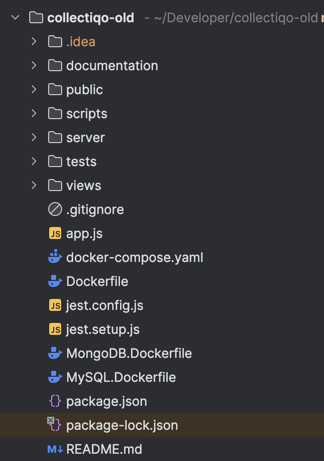
\includegraphics[width=0.5\textwidth]{root_path_structure_old}
  \caption{Old root path structure}
  \label{fig:root_path_structure_old}
\end{figure}
\begin{figure}[h]
  \centering
  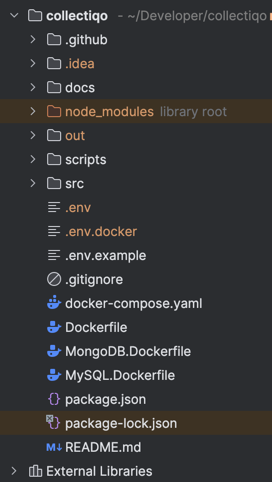
\includegraphics[width=0.5\textwidth]{root_path_structure_new}
  \caption{New root path structure}
  \label{fig:root_path_strucutr_new}
\end{figure}
Code, der zuvor unter den Ordnern Server, Public und Views zu finden war, wurde nun in den src Ordner verlagert.
Im nächsten Abschnitt wird der Inhalt des src Ordners genauer betrachtet.

\subsubsection{Struktur des Quellcodes}
Wie zuvor beschrieben beinhaltet der src Ordner jegliche Dateien, die den Quellcode der Collectiqo App beinhalten.
Hierzu zählen ebenfalls einige Ordner wie der public und views Ordner, die zuvor auf root Ebene vorhanden waren.
Hier eine Übersicht über alle Inhalte des neuen src Ordners:
\begin{figure}[h]
  \centering
  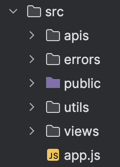
\includegraphics[width=0.5\textwidth]{src_folder_structure}
  \caption{src Folder Structure}
  \label{fig:src_folder_structure}
\end{figure}

Während zuvor alle Bestandteile einer Funktion (Route, Response Codes und Funktionalität) in einer Datei gehandhabt wurden, wurden diese nun in drei separate Dateien aufgeteilt.
Jede Route erhält eine eigene Datei, in welcher der Endpunkt für HTTP Request definiert wird und der entsprechende Controller aufgerufen wird.
Hier ein Beispiel für die Route der Login Funktion:
\lstset{language=javascript}
\begin{lstlisting}[label={lst:lst-login-route}]
const express = require('express');
const router = express.Router();
const loginController = require('../controllers/loginController');

router.post('/login', loginController);

module.exports = router;
\end{lstlisting}


Der Controller kümmert sich um den Aufruf der gewünschten Service Datei und handhabt die Response Codes, die beim Aufruf des Endpunkts zurückgegeben werden.
Als Beispiel dient dieser Controller der Login Funktion:

\begin{lstlisting}[label={lst:lst-login-controller}]
const loginService = require('../services/loginService');

// Extract constants for response messages
const LOGIN_SUCCESS_MESSAGE = 'Login successful';
const INTERNAL_SERVER_ERROR_MESSAGE = 'Internal server error';

// Extract error handling into a separate function
const handleLoginError = (res, error) => {
  console.error('Login error:', error);
  res.status(500).json({message: INTERNAL_SERVER_ERROR_MESSAGE});
};

const loginController = async (req, res) => {
  const {username, password} = req.body;
  try {
    // check if user can be found in database
    const user = await loginService(username, password);
    // throw error if user can't be found
    if(user===undefined){
      throw new Error('User not found')
    }
    // add user data to session variables
    req.session.user = {
      name: user.username,
      id: user.id,
      isLoggedIn: true
    }

    // try to save changes, else throw error
    try {
      await req.session.save();
      console.log(`User ${req.session.user.name} logged in successfully`);
      res.status(200).json({message: LOGIN_SUCCESS_MESSAGE, userId: req.session.user.id});
    } catch (err) {
      console.error('Error saving to session storage: ', err);
      return new Error('Error logging in user');
    }
  } catch (error) {
    handleLoginError(res, error);
  }
};

module.exports = loginController;
\end{lstlisting}

Die eigentliche Funktionalität ist in der Service Datei implementiert.
Zuletzt noch die Service Datei der Login Funktion:

\begin{lstlisting}[label={lst:lst-login-service}]

const bcrypt = require('bcryptjs');
const { queryDatabase, handleResults } = require('../../../utils/mysqlUtils');

const loginService = async (username, password) => {
    const results = await queryDatabase('SELECT * FROM clq_users WHERE username = ? OR email = ?', [username, username]);
    const user = handleResults(results);

    if (!user) {
        throw new Error('User not found');
    }

    const passwordMatches = await bcrypt.compare(password, user.password);
    if (!passwordMatches) {
        throw new Error('Incorrect password');
    }

    return user; // Ensure the user object is returned
};

module.exports = loginService;
\end{lstlisting}

Diese Aufteilung bringt mehrere Vorteile mit sich.
Jede Funktionalität, die ab sofort implementiert wird, folgt genau diesem Muster, wodurch jede Implementierung für jedes Teammitglied klar nachverfolgbar ist.
Darüber hinaus erleichtert es das Debugging ungemein, da Probleme einfacher auf einzelne Bestandteile eines Funktionsaufrufs zurückgeführt werden können.
Kombiniert mit einer Ordnerstruktur, die inhaltlich ferne Funktionen voneinander trennt, ist auf das Navigieren innerhalb des Projekts vereinfacht.
Schlussendlich ist auch das Aufrufen vom HTTP Requests vereinfacht, da jeder Aufruf einheitlich ist.